\section{Getting Started}
This section describes how to load the FPGA bitstream on an empty CMOD-A7 board.
\paragraph{Requirements}~\\
The following resources and pieces of software are needed:
\begin{itemize}
    \item the HTMega-FPGA project, containing design sources and configurations
    \item the Vivado-ML IDE (more details in \cite{vivado} - \citetitle{vivado})
    \item the CMOD A7 board files (more details in \cite{cmod-a7-board-files} - \citetitle{cmod-a7-board-files})
\end{itemize}
The standard version of Vivado is free to use, but requires a Xilinx account.

\paragraph{Generating Bitstream}~\\
Open the HTMega\_FPGA.xpr file inside the project folder.
Even though the project folder contains the finished bitstream, it is recommended to generate a bitstream after opening the project for the first time by clicking on 'generate bitstream' on the left panel.
This will also launch synthesis and implementation. Click on 'Yes' or 'OK' when Vivado asks if you want to launch Synthesis and Implementation.\\
This might take, depending on your pc, 10 - 20 minutes.  

\paragraph{Connecting to the Target}~\\
Once the bitstream generation is finished, a dialog will pop up asking if you want to open the hardware manager, click yes.
If you want to open the hardware manager afterwards, click 'open hardware manager' below.
After opening the hardware manager, click on 'Open Target' and 'Auto Connect' in the top bar.
\pagebreak


\paragraph{Volatile Programming}~\\
Programming the Artix-7 over JTAG will only load the bitstream onto the FPGA, which is volatile. Thus, once you remove the power, the FPGA configuration will be lost.
To program the FPGA over JTAG, right-click on the Artix-7 device and click on 'Program Device'.
\begin{figure}[h]
    \center
    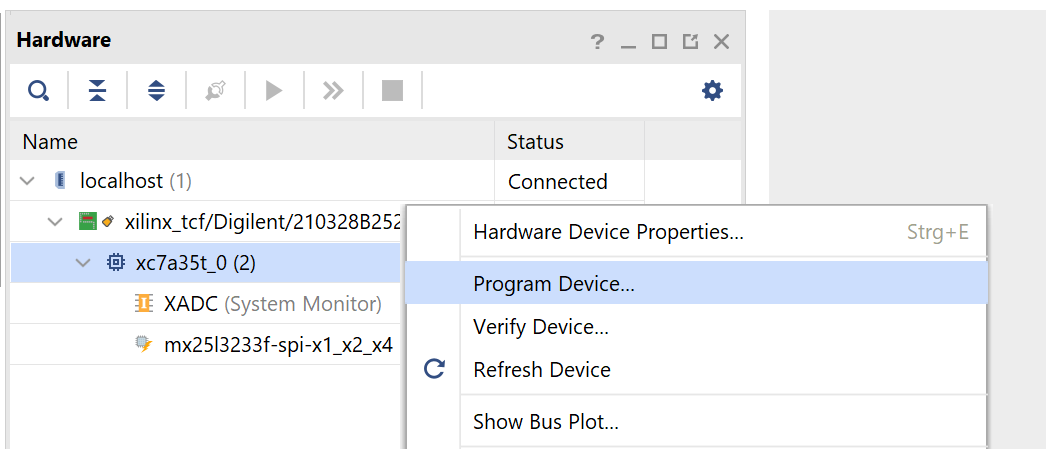
\includegraphics[scale=0.8]{assets/jtag-programming.png}
    \caption{Programming over JTAG}
\end{figure}\\
This might take up to a minute.

\paragraph{Nonvolatile Programming}~\\
To make the FPGA configuration constant, the bitstream will have to be loaded onto the onboard flash. The Artix-7 will then load the bitstream from the flash on every startup.
To load the bitstream onto the flash, right-click on the memory device and click on 'Program Configuration Memory Device'.
\begin{figure}[h]
    \center
    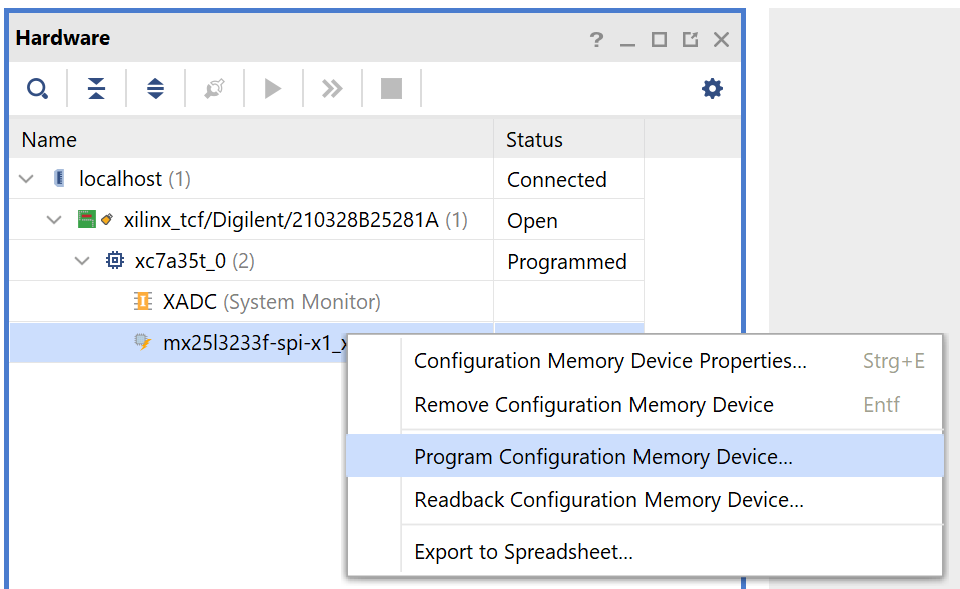
\includegraphics[scale=0.8]{assets/spi programming.png}
    \caption{Programming the configuration memory device}
\end{figure}~\\
This will take a lot longer than JTAG programming, but once the flash is programmed, every startup will only take a few milliseconds.
